% !TeX root = ../main.tex
\section{Study region and data}
\subsection{Balsa plantation inventory}

The study covered mainland Ecuador, with particular emphasis on the humid Pacific lowlands and western Andean foothills where commercial BALSA plantations are concentrated as shown in Fig.~\ref{fig:study_area}. Balsa plantation boundaries were obtained from the Ecuadorian Ministry of Agriculture and Livestock through the Geoportal del Agro Ecuatoriano (\url{https://geoportal.agricultura.gob.ec/}).

\begin{figure}[pos=!htbp]
    \centering
    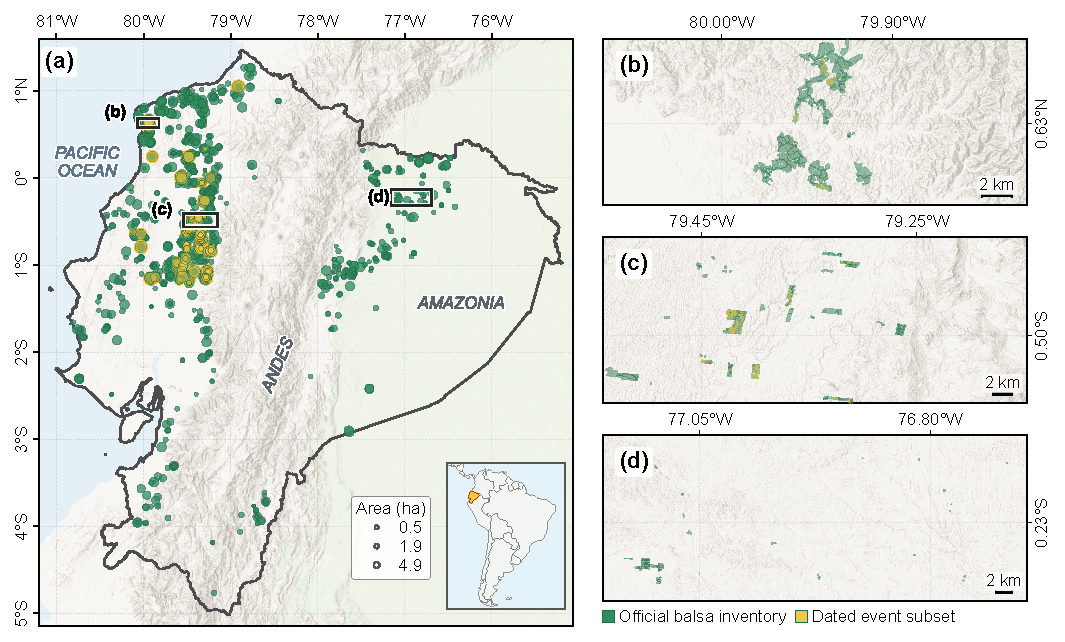
\includegraphics[width=0.92\linewidth]{figures/fig02_study_area.pdf}
    \caption{Study region and official BALSA plantation inventory. Green markers show all 3,890 BALSA polygons, and yellow markers identify the subset containing dated stand-disturbance events. (b)--(d) enlarge representative plantation regions.}
    \label{fig:study_area}
\end{figure}

The source forestry inventory contained 26,206 plantation polygons, of which 3,498 carried the species label BALSA and marked VALIDADO. The validated balsa inventory covered 13,651.85~ha and was divided into three fixed size classes for stratified reporting: small ($\leq1$~ha), medium ($>1$--5~ha), and large ($>5$~ha) (Table~\ref{tab:inventory}).

\begin{table}[pos=!htbp]
    \centering\small
    \caption{Area characteristics of the 3,498 retained BALSA polygons.}
    \label{tab:inventory}
    \begin{tabular}{lrrrrr}
    \toprule
    Area class & Polygons & Count (\%) & Area (ha) & Area (\%) & Median (ha)\\
    \midrule
    Small ($\leq1$ ha) & 1,325 & 37.88 & 497.38 & 3.64 & 0.30\\
    Medium ($>1$--5 ha) & 1,385 & 39.59 & 3,556.10 & 26.05 & 2.33\\
    Large ($>5$ ha) & 788 & 22.53 & 9,598.37 & 70.31 & 8.68\\
    \bottomrule
    \end{tabular}
\end{table}

\subsection{Near-decadal Sentinel-1 observation design}
\label{sec:observation_design}

We used VV and VH backscatter from the OPERA radiometric Sentinel-1 observations were obtained from the NASA OPERA Level-2 Radiometric Terrain Corrected Sentinel-1 (RTC-S1) archive~\citep{shiroma2023OPERARTC,opera2023rtc} and organized using S1-GRiTS v3.0.0 (\url{https://github.com/ottoKae/S1-GRiTS}). OPERA RTC-S1 provides burst-based, radiometrically terrain-corrected $\gamma^{0}$ backscatter at 30-m pixel spacing for VV and VH polarizations.

% 说明组织数据的数量级别
As shown in Table~\ref{tab:s1_observation_coverage}, the Ecuadorian Sentinel-1 SAR archive was organized by four ascending relative-orbit tracks (TK18, TK47, TK91, and TK120). The archive was queried from January 2016 to June 2026, while the first available observations for individual tracks occurred between May and October 2016. In total, 71,134 burst-level RTC products were available, providing dense long-term coverage while preserving track identity throughout subsequent processing.  Detailed acquisition-level compositing, missing-data handling, and stand-level aggregation are described in Section~\ref{sec:s1_timeseries_representation}.

% The 3,498 validated BALSA polygons intersected 40 tile--track combinations, yielding 4,001 polygon--track objects for time-series extraction. Track identity was preserved throughout time-series construction and disturbance detection so that observations from different relative orbits or viewing geometries were not mixed before event consolidation.

\begin{table*}[pos=!htbp]
    \centering
    \small
    \setlength{\tabcolsep}{6pt}
    \caption{Track-specific Sentinel-1 RTC observation coverage used to construct stand-level time series. The archive includes 40 tile--track groups across 31 unique MGRS tiles.}
    \label{tab:s1_observation_coverage}

    \begin{tabular*}{\linewidth}
        {@{\extracolsep{\fill}}lrlrr@{}}
        \toprule
        Track &
        Tile--track groups &
        Observation span &
        RTC burst products &
        stand-level trajectories \\
        \midrule
        TK18  & 19 & Sep. 2016--Jun. 2026     & 36,006 & 3,467 \\
        TK47  & 2  & Jun. 2016--Jun. 2026     & 3,664  & 16    \\
        TK91  & 5  & Oct. 2016--Jun. 2026     & 7,648  & 61    \\
        TK120 & 14 & May. 2016--Jun. 2026     & 23,816 & 457   \\
        \midrule
        Total & 40 & May. 2016--Jun. 2026 &
        \textbf{71,134} & \textbf{4,001} \\
        \bottomrule
    \end{tabular*}
\end{table*}

\subsection{Dated reference events}

Historical disturbance months were assigned by visual interpretation and reconciled to the frozen polygon identifiers. Single-date PlanetScope imagery (approximately 3~m) was the primary evidence source, with monthly Planet basemaps (approximately 4.77~m at the Equator) used where appropriate (Fig~\ref{fig:s1_population_signatures}). Orbit-specific Sentinel-1 observations provided supplementary evidence when cloud cover or incomplete optical observations prevented an unambiguous optical-only date assignment. Interpretation was performed without access to Windowed CUSUM predictions, and ambiguous disturbance dates were not forced into the reference catalogue. After exact polygon--month duplicates were reconciled, the historical catalogue contained 1,093 reference-dated events in 462 validated BALSA polygons distributed across 57 spatial blocks within the 2017--2025 historical evaluation period.